\documentclass{article}

% Language and font encodings
\usepackage[english]{babel}
\usepackage[utf8x]{inputenc}
\usepackage[T1]{fontenc}
\usepackage{verbatim} % multiline comments

% Sets page size and margins
\usepackage[a4paper,top=3cm,bottom=2cm,left=3cm,right=3cm,marginparwidth=1.75cm]{geometry}

% Useful packages
\usepackage{amsmath}
\usepackage{float}
\usepackage{rotating}
\usepackage{booktabs}
\usepackage{graphicx}
\usepackage[colorinlistoftodos]{todonotes}
\usepackage[colorlinks=true, allcolors=blue]{hyperref}
\usepackage[round]{natbib}
\usepackage[switch]{lineno} % line numbers
\usepackage{longtable}
\usepackage{multirow}
\usepackage{ulem}

% Supplementary Materials
\newcommand{\beginsupplement}{
	\setcounter{table}{0}
	\renewcommand{\thetable}{S\arabic{table}}
	\setcounter{figure}{0}
	\renewcommand{\thefigure}{S\arabic{figure}}
}

\title{Dewlap color variation in \textit{Anolis sagrei} is maintained among habitats within islands of the West Indies}

\date{}

\begin{document}
	
	\linenumbers
	
	\maketitle
	
	\begin{abstract}
		Animal signals evolve in an ecological context. Moreover, locally adapting animal sexual signals can be especially important for initiating or reinforcing reproductive isolation during the early stages of speciation. Dewlap color in \textit{Anolis} lizards can be highly variable between populations in relation to both biotic and abiotic adaptive drivers, albeit at relatively large geographical scales. Here, we investigated local adaptation of the dewlap across habitat-types at a small spatial scale, as this may give an indication of how conditions for the early stages of speciation may be met. We explored variation in dewlap coloration in the most widespread species of anole, \textit{Anolis sagrei}, across three characteristic habitats spanning the Bahamas and the Cayman Islands. Using reflectance spectrometry as well as supervised machine learning, we found some consistent differences in spectral properties of the dewlap between habitats within small islands. Passive divergence in dewlap phenotype associated with isolation-by-distance did not explain our results. Instead, the observed patterns in dewlap coloration are more consistent with an adaptive explanation in these \textit{A. sagrei} populations, as one would otherwise expect differences within islands to be erased by gene flow at such small geographical scales. Although these habitat-specific dewlap differences vary in magnitude and direction across islands, and islands themselves differ substantially, we found a suite of consistent archipelago-wide differences between habitat types, suggesting parallel responses to similar selective pressures. While at present, populations from these different habitats probably experience too much gene flow to follow distinct evolutionary lineages, should additional barriers arise between habitat-specific populations, the observed disruptive selection on dewlap coloration may facilitate ecological speciation.
	\end{abstract}
	
	\textbf{Keywords} --- reflectance, adaptation, sexual signal, machine learning, polymorphism
	
	\pagebreak
	
	\section*{Introduction}
	
	The staggering diversity of animal communication signals has long been of interest to evolutionary biologists. Animals use chemical, mechanical, electromagnetic, and visual signals to communicate in a wide variety of contexts, including, competition for mates, species recognition, aposematism, and cooperation \citep{Bradbury2011}. A primary evolutionary factor shaping communication signals is the sensory system and behavior of recipients (the sensory drive hypothesis; \citealt{Endler1988,Endler1992,Endler1998}). Over the past decades, scientists have established that signals evolve in an ecological context and are dependent on environmental conditions \citep{Endler1992,Endler1993,Endler1993a}. Just as different habitats may favor different combinations of ecomorphological traits to maximize performance and fitness \citep{Arnold1983}, they may also shape different forms of a signal, so as to maximize its transmission and detection (e.g. \citealt{Seehausen1997}), or reduce its detection by unintended recipients such as predators \citep{Endler1984,Endler1990,Endler1991,Halfwerk2014}. This selective pressure may drive the local adaptation of communication signals.\\

One potential barrier to the maintenance of localized signal divergence is the homogenizing effect of gene flow. Population genetics theory suggests that gene flow may counteract local adaptation between localities and prevent divergence altogether, especially at small spatial scales, because of the inflow of maladapted alleles or because of the breaking of linkage between coevolving loci \citep{Felsenstein1976, Garcia-Ramos1997, Dieckmann1999, Lenormand2002, Hendry2007}. This genetic homogenization has been confirmed empirically in systems such as stick insects \citep{Nosil2004} and stickleback \citep{Hendry2007a}. Yet, examples of microgeographic adaptation, i.e. adaptation at smaller scales than the range of dispersal, exist, highlighting the potential of some organisms to respond to selection in the face of gene flow (see \citealt{Richardson2014} and references therein). Examples include small scale adaptation in fragmented areas in Australian fruit flies \citep{Willi2012}, and local adaptation to predation pressure in North American salamanders \citep{Richardson2013}. Therefore, despite evidence that local adaptation may be particularly difficult at small spatial scales where gene flow tends to cause adjoining populations to remain genetically homogeneous, the potential adaptive response of species traits, in particular communication signals, to localized differences in habitats remains relatively unknown \citep{Richardson2014}. Lizards of the neotropical genus \textit{Anolis} (Squamata: Dactyloidae) are an excellent group for studying the eco-evolutionary dynamics of local adaptation and natural selection \citep{Losos2009}. A particularly conspicuous trait of anoles is their dewlap, an extensible flap of skin that is typically sexually dimorphic and used as a communication signal in courtship \citep{Sigmund1983, Driessens2014, Driessens2015} and territorial displays \citep{Losos1985, Macedonia1994, Macedonia2013} as well as in predator deterrence \citep{Leal1995, Leal1997, Leal1997a}. Dewlap characteristics vary widely among the approximately $400$ species of the genus \citep{Nicholson2007}. Interspecific variation in dewlap coloration is implicated in species recognition \citep{Rand1970, Williams1969, Williams1977, Losos1985, Macedonia1994, Fleishman2000, Macedonia2013}, and this function could have had a role in initiating or reinforcing reproductive isolation during speciation \citep{Lambert2013, Geneva2015, Ng2017}.\\

Within species, studies have shown a link between variation in dewlap coloration and differences in habitats or climatic conditions \citep{Macedonia2001, Leal2002, Thorpe2002, Thorpe2002a, Leal2004, Vanhooydonck2009, Ng2012, Ng2013, Ng2016, Vanhooydonck2009, Driessens2017}. Some studies suggest that those differences may be adaptive and that dewlaps may have evolved to maximize detectability given local light conditions \citep{Fleishman2001, Leal2002, Leal2004}. Although this claim is further supported by recent findings that dewlap colors are perceived differently under different levels of shading \citep{Fleishman2020}, other studies found conflicting patterns of between-habitat variation that did not support the sensory drive hypothesis \citep{Fleishman2009, Ng2012, Macedonia2014}.\\ 

Previous studies investigating variation in anole dewlaps compared populations at relatively large geographical scales, e.g. between islands \citep{Vanhooydonck2009, Driessens2017} or within large islands such as Puerto Rico \citep{Leal2004} or Hispaniola \citep{Ng2012, Ng2016}. These large scales and marine barriers should reduce gene flow \citep{Ng2011, Lambert2013, Richardson2014, Ng2017}. That said, examples do exist of divergence in dewlap coloration at smaller scales or between populations with high degrees of gene flow \citep{Thorpe2002, Thorpe2002a, Stapley2011, Ng2016}.\\

\textit{Anolis sagrei} is widespread across islands of the West Indies \citep{Reynolds2020}. It has been the subject of numerous studies concerning local adaptation \citep{Losos1994, Losos1997a, Losos2001, Kolbe2012}, biological invasion \citep{Kolbe2008}, and sexual selection \citep{Tokarz2002, Tokarz2005, Tokarz2006, Driessens2014, Steffen2014, Driessens2015} among many other topics. Between-island variation in the mainly orange-red color of its dewlap was shown to be better explained by climatic variables such as annual precipitation and solar radiation (proposed to affect the average vegetation type on each island and among other things, its ambient light environment, \citealt{Driessens2017}),  than by proxies for biotic factors such as sexual selection or predation pressure \citep{Vanhooydonck2009, Baeckens2018}. How intra-island differences in habitat may contribute to the diversity of dewlap coloration, however, remains unexplored, and may reveal new insights into the scale of local differentiation despite gene flow.\\

Here, we analyzed the color characteristics of \textit{A. sagrei} dewlaps within nine islands in the Bahamas and Cayman Islands. These island systems presently, if not historically, comprise relatively small islands, with no major geographic barriers within islands limiting dispersal for this species. These islands all share three characteristic native West Indian small-island habitat-types -- beach scrub bush, closed-canopy primary coppice forest, and mangrove forest -- that are often spatially intermingled. These habitats contrast in environmental parameters including vegetation community, light irradiance, humidity, and temperature \citep{Howard1950, Schoener1968}. The Cayman Islands and the Bahamas have been colonized independently by \textit{A. sagrei} from Cuba (\citealt{vandeSchoot2016} unpublished thesis; \citealt{Reynolds2020}), such that these archipelagos constitute an ideal suite of natural replicates to explore within-island dewlap diversity across multiple islands.\\

Our sampling design included sites in close proximity; the median distance between two sites within an island was \sout{$11.2$} \textcolor{olive}{8.45}km. While this species has traditionally been considered territorial, a recent study revealed that they are polygynandrous and that gene flow is not impeded by territorial-like behaviors exibited by some males (Kamath and Losos 2018). Combining reflectance spectrometry and supervised machine learning, we tested for divergence in dewlap phenotype between habitats within islands and between islands across part of the range of \textit{A. sagrei}. We predicted that if light conditions in the environment indeed drive color evolution, dewlaps should be most similar between beach scrub and mangrove forest, which both have high levels of light irradiance, compared to the darker, closed-canopy coppice forest. If detectability is maximized given the local conditions, we expected darker and more contrasting dewlaps in high irradiance habitats. Finally, if habitat characteristics are strong determinants of dewlap color variation, similar patterns should be observed across multiple islands \citep{Harvey1991, Losos2011}.
	
	\pagebreak
	
	\section*{Methods}
	
	\input{sections/methods_tracked.tex}
	
	\pagebreak
	
	\section*{Results}
	
	We tested for variation in \textit{A. sagrei} dewlap coloration between populations living in three characteristic habitat types across nine islands that span the West Indian range of the brown anole (beach scrub, primary coppice and mangroves). We found that most of the variation in coloration was partitioned between islands (two-way PERMANOVA, \sout{$F(df = 8) = 43.7$, $P = 0.0001$} \textcolor{olive}{$F(df = 8) = 45.38$, $P = 0.001$}, explained variance \sout{$R^2 = 40.9$} \textcolor{olive}{$R^2 = 41.4$}\%). Nonetheless, we did find evidence for differences in dewlap coloration between habitat types, and those were mostly island-specific (habitat-by-island interaction term, \sout{$F(16) = 3.53$, $P = 0.0001$, $R^2 = 6.6$} \textcolor{olive}{$F(16) = 4.78$, $P = 0.001$, $R^2 = 8.7$}\%), with a significant portion of the variation explained by an habitat effect across all islands, but this effect was relatively small (\sout{$F(2) = 4.7$, $P = 0.0001$, $R^2 = 1.1$} \textcolor{olive}{$F(2) = 4.46$, $P = 0.001$, $R^2 = 1$}\%).\\

We subsequently tested for differences in dewlap coloration between habitat-populations within each island, using within-island principal component scores (to maximize the variation captured for each island, see Methods). Our within-island random forest classification analyses revealed detectable differences in dewlap coloration on \sout{eight} \textcolor{olive}{seven} out of the nine islands in our sample: Abaco, Bimini, Cayman Brac, Eleuthera, Little Cayman, Long Island, \textcolor{olive}{and} North Andros \sout{and South Andros}. The accuracy of random forest classification exceeded random expectation more often than expected by chance for all these islands (Table \ref{tab:randomforests}). Accuracy was as high as \sout{73} \textcolor{olive}{74.8}\% for Cayman Brac. We obtained similar results using other machine learning approaches such as support vector machines (Table \ref{tab:ksvms}) and linear discriminant analysis (Table \ref{tab:ldas})\sout{, except that these methods did not detect significant differences on Eleuthera and North Andros}. We describe in details the specific differences detected on each island in the Appendix, and focus here on the general patterns emerging from our data.\\

Overall, we found significant differences in dewlap coloration between populations that were often in close geographical proximity. On Bimini, notably, we found a significant difference between dewlaps from beach scrub and primary coppice forest, at a distance of a few hundred meters, making this contrast the smallest geographical scale at which differences in coloration were found in our study (Fig. \ref{fig:Bimini}). We also detected significant differences in dewlap coloration at distances below one kilometer on Abaco (Fig. \ref{fig:Abaco_supplement}G), and at distances between one and ten kilometers on Bimini (Fig. \ref{fig:Bimini}G), Cayman Brac (Fig. \ref{fig:CaymanBrac}G), Little Cayman (Fig. \ref{fig:LittleCayman}G), Long Island (Fig. \ref{fig:LongIsland}G) and \sout{South} \textcolor{olive}{North} Andros (Fig. \ref{fig:NorthAndros}G).\\

We found evidence of spatial autocorrelation in dewlap coloration between the sites within islands for Abaco (Table \ref{tab:autocorrelation}), suggesting that populations from closer sites tend to have more similar dewlaps on this island than expected by chance. Abaco was the island we sampled at the largest scale, with some sites nearly a hundred kilometers away from each other (Fig. \ref{fig:Abaco}A). That said, some sites were also in close proximity, and significant differences in coloration were detected between habitats sometimes less than a kilometer away (Fig. \ref{fig:Abaco_supplement}G), suggesting that differences in dewlap coloration between distant sites may be partly attributable to isolation-by-distance, but this may not necessarily be the case for sites in close proximity. We did not find evidence for spatial autocorrelation on other islands than Abaco (although Eleuthera was nearly significant, Table \ref{tab:autocorrelation}).\\

A striking feature of our data was inconsistency in between-habitat differences among islands, in terms of which habitats differ from which, which dimensions of coloration were involved, and in which direction. For example, while on Cayman Brac the random forests could well distinguish between all three habitats (Fig. \ref{fig:CaymanBrac}D), on Abaco dewlaps from beach scrub and primary coppice were often mistaken, and on Bimini beach scrub dewlaps were more often classified into primary coppice or mangrove than into beach srub (Fig. \ref{fig:Bimini}D). In terms of variable importance, for multiple islands the random forests used information in the UV range to discriminate between at least some habitats, particularly on Abaco (Fig. \ref{fig:Abaco_supplement}F), Bimini (Fig. \ref{fig:Bimini}F), Cayman Brac (Fig. \ref{fig:CaymanBrac}F), Little Cayman (Fig. \ref{fig:LittleCayman}F) and Long Island (Fig. \ref{fig:LongIsland}F), but differences in UV reflectance involved different habitats and were in different directions among these islands.\\
	
	\pagebreak
	
	\section*{Discussion}
	
	\input{sections/discussion_tracked.tex}
	
	\pagebreak
	
	\bibliographystyle{apalike}
	\bibliography{library.bib}
	
	\pagebreak
	
	\section*{Figures}
	
	\pagebreak
	
	% Map of the West Indies
\begin{figure}[H]
    \centering
	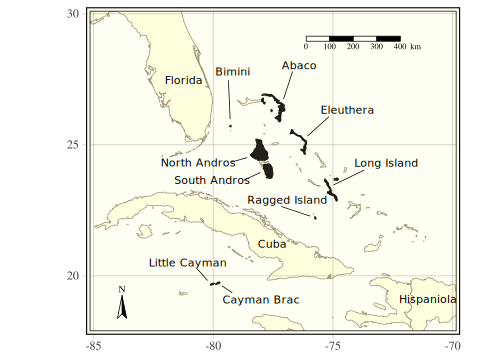
\includegraphics[width=0.8\textwidth]{figures/map.pdf}
	\caption{Map of the West Indies with sampled islands highlighted in black.}
	\label{fig:map}
\end{figure}

% Classification accuracy of SVMs
\begin{figure}[H]
    \centering
	\includegraphics[width=\textwidth]{figures/classif_svm_pca.png}
	\caption{Distributions of classification accuracy across all SVM machines (100 replicates of 5 cross-validation bins each). The dashed line represents the density of a corresponding null binomial distribution, which would be expected under random guessing (testing sets with 20\% of the observations for each island and success probability of $1/3$). Inset plots show the corresponding average confusion matrices and represent the proportion of lizards from each habitat (columns) reassigned in each other habitat (rows), with an interpretation guide in the right panel. P-values indicate deviations of the mean classification accuracy to the expected null binomial distribution. *, P < 0.05}
	\label{fig:classif_svm_pca}
\end{figure}

% Boxplots and analyses of variance
\begin{sidewaysfigure}
    \centering
	\includegraphics[width=18cm]{figures/figure_anova.png}
	\caption{Dewlap coloration varies between habitat-types along different dimensions on different islands. (A) Boxplots show the distribution of the data for the five islands with significant differences in dewlap coloration between habitat (P-values in Fig. \ref{fig:classif_svm_pca}), along the first four principal components. We report the P-values of univariate analyses of variance conducted for each island (see Methods). Horizontal bars indicate \textit{post hoc} significant contrasts at a 0.05 error rate (see Methods). *, P < 0.05. (B) Mapping of the reflectance at various wavelengths onto the principal components. Note that PC1 largely represents brightness.}
	\label{fig:boxplots}
\end{sidewaysfigure}
	
	\pagebreak
	
	\section*{Tables}
	
	\pagebreak
	
	\begin{sidewaystable}
	\label{tab:anova}
	\caption{Significance of habitat differences in dewlap coloration, using ANOVA for all islands where significant multivariate differences in dewlap coloration were detected by SVMs. Best fitting model: 1, OLS; 2, GLS. df, degrees of freedom. $\Delta$AICc, difference in AICc between the best fitting model and the OLS-model. AICcw, AICc weight. LRT, likelihood ratio test. Log-lik., log-likelihood. $\chi^2$, likelihood ratio. *, P < 0.05; **, P < 0.01, ***, P < 0.001.}
	\centering
	
\begin{tabular}{llrrrrrrrrrl}
\toprule
nesting & variable & best\_fit & df\_model & AICc & dAICc & AICcw & df\_LRT & loglik & lratio & pvalue & signif\\
\midrule
Abaco & PC1 & 1 & 4 & 710.4 & 0.0 & 0.746 & 2 & -357.0 & 0.14 & 0.9308 & \\
Abaco & PC2 & 1 & 4 & 620.1 & 0.0 & 0.882 & 2 & -310.2 & 31.74 & 0.0000 & ***\\
Abaco & PC3 & 1 & 4 & 517.8 & 0.0 & 0.732 & 2 & -257.2 & 27.37 & 0.0000 & ***\\
Abaco & PC4 & 1 & 4 & 440.6 & 0.0 & 0.596 & 2 & -217.2 & 1.36 & 0.5070 & \\
Bimini & PC1 & 1 & 4 & 561.3 & 0.0 & 0.595 & 2 & -283.1 & 7.40 & 0.0248 & *\\
\addlinespace
Bimini & PC2 & 1 & 4 & 448.1 & 0.0 & 0.656 & 2 & -223.8 & 8.09 & 0.0175 & *\\
Bimini & PC3 & 2 & 6 & 405.3 & -0.2 & 0.529 & 2 & -199.2 & 10.39 & 0.0056 & **\\
Bimini & PC4 & 1 & 4 & 274.2 & 0.0 & 0.854 & 2 & -132.7 & 0.33 & 0.8499 & \\
Cayman Brac & PC1 & 2 & 6 & 402.8 & -4.1 & 0.884 & 2 & -200.9 & 13.81 & 0.0010 & **\\
Cayman Brac & PC2 & 1 & 4 & 332.1 & 0.0 & 0.853 & 2 & -165.9 & 8.41 & 0.0149 & *\\
\addlinespace
Cayman Brac & PC3 & 1 & 4 & 295.8 & 0.0 & 0.800 & 2 & -146.6 & 27.16 & 0.0000 & ***\\
Cayman Brac & PC4 & 1 & 4 & 279.2 & 0.0 & 0.897 & 2 & -137.8 & 5.63 & 0.0600 & \\
Little Cayman & PC1 & 1 & 4 & 367.2 & 0.0 & 0.777 & 2 & -186.0 & 8.18 & 0.0167 & *\\
Little Cayman & PC2 & 2 & 6 & 287.6 & -3.6 & 0.859 & 2 & -140.5 & 29.76 & 0.0000 & ***\\
Little Cayman & PC3 & 1 & 4 & 277.7 & 0.0 & 0.669 & 2 & -138.1 & 21.34 & 0.0000 & ***\\
\addlinespace
Little Cayman & PC4 & 1 & 4 & 226.7 & 0.0 & 0.780 & 2 & -110.7 & 2.85 & 0.2410 & \\
Long Island & PC1 & 2 & 6 & 442.3 & -2.1 & 0.740 & 2 & -221.2 & 2.91 & 0.2331 & \\
Long Island & PC2 & 2 & 6 & 351.4 & -3.1 & 0.823 & 2 & -172.6 & 4.52 & 0.1043 & \\
Long Island & PC3 & 1 & 4 & 322.1 & 0.0 & 0.862 & 2 & -160.0 & 11.24 & 0.0036 & **\\
Long Island & PC4 & 1 & 4 & 195.5 & 0.0 & 0.767 & 2 & -92.9 & 6.46 & 0.0395 & *\\
\bottomrule
\end{tabular}

\end{sidewaystable}




	
	\pagebreak
	
	\beginsupplement
	
	\pagebreak
	
	\section*{Appendix}
	
	\input{sections/appendix_tracked.tex}
	
	\pagebreak
	
	\section*{Supplementary Figures}
	
	\pagebreak
	
	\input{sections/suppfigures_tracked.tex}
	
	\pagebreak
	
	\section*{Supplementary Tables}
	
	\pagebreak
	
	\begin{table}
	\label{suptab:counts}	
	\caption{Number of lizards sampled in each habitat on each island.}
	\centering
	% Sample sizes
\begin{table}[H]
    \caption{Numbers of lizards sampled across islands and habitats.}
    \centering
    \begin{tabular}{lrrr}
        \hline
        & coastal & coppice & mangrove\\
        \hline
        Abaco & 41 & 24 & 21\\
        Bimini & 38 & 14 & 15\\
        Cayman Brac & 15 & 18 & 17\\
        Eleuthera & 22 & 25 & 9\\
        Little Cayman & 17 & 12 & 16\\
        Long Island & 26 & 14 & 13\\
        North Andros & 9 & 9 & 10\\
        Ragged Island & 18 & 15 & 17\\
        South Andros & 10 & 9 & 12\\
        \hline
    \end{tabular}
    \label{suptab:counts}
\end{table}
\end{table}

\begin{table}
	\label{suptab:sites}
	\caption{Locations of the sampling sites across islands, with mean principal component scores per site.}
	\centering
	
\begin{tabular}{lrrlrrrr}
\toprule
Island & Longitude & Latitude & Habitat & PC1 & PC2 & PC3 & PC4\\
\midrule
Abaco & -77.7256 & 26.9083 & mangrove & -5.4905 & 1.3541 & -0.4741 & 0.0083\\
Abaco & -77.5800 & 26.9020 & coastal & 1.8633 & 0.0365 & -0.4475 & 0.0033\\
Abaco & -77.5763 & 26.9128 & coppice & -1.6738 & -1.7793 & -0.0499 & 0.0012\\
Abaco & -77.1784 & 26.1045 & coastal & 1.1863 & 2.0408 & -0.3468 & 0.0022\\
Abaco & -77.0055 & 26.3254 & mangrove & -9.0319 & -2.7460 & 0.4687 & 0.0077\\
Abaco & -77.0039 & 26.3170 & coppice & 0.9967 & 0.5161 & -0.0267 & -0.0118\\
Abaco & -76.9968 & 26.3260 & coastal & 7.6077 & 0.3186 & 0.1771 & -0.0008\\
Bimini & -79.3022 & 25.5859 & coastal & 5.7537 & -0.1593 & -0.2505 & 0.0001\\
Bimini & -79.3014 & 25.7052 & coastal & -3.1822 & 1.6617 & -0.0460 & 0.0024\\
Bimini & -79.3002 & 25.7042 & coppice & -1.3514 & -3.8786 & 0.1027 & -0.0027\\
Bimini & -79.2709 & 25.7066 & mangrove & 3.3656 & 0.6244 & 0.1569 & -0.0021\\
Cayman Brac & -79.8627 & 19.6878 & coastal & 6.6606 & -2.5670 & 0.0166 & -0.0007\\
Cayman Brac & -79.8441 & 19.6949 & mangrove & -1.0914 & 4.3607 & 0.0855 & 0.0001\\
Cayman Brac & -79.7887 & 19.7209 & coppice & -4.5197 & -1.9793 & -0.0946 & 0.0004\\
Eleuthera & -76.3347 & 24.8146 & coppice & 3.2669 & -1.2404 & 0.1018 & -0.0085\\
Eleuthera & -76.3058 & 24.8127 & coastal & 0.4216 & -3.5133 & -0.0567 & 0.0009\\
Eleuthera & -76.2901 & 24.7981 & mangrove & 2.1881 & 0.7517 & 0.3957 & -0.0055\\
Eleuthera & -76.1616 & 24.9129 & coppice & -1.9136 & 1.0868 & -0.4978 & -0.0092\\
Eleuthera & -76.1492 & 24.9335 & coastal & -3.1863 & 2.4270 & 0.1881 & 0.0218\\
Little Cayman & -80.0660 & 19.6906 & coppice & 0.8021 & -1.9569 & -0.0760 & -0.0068\\
Little Cayman & -80.0205 & 19.6865 & coastal & -6.6917 & -1.2615 & 0.0659 & 0.0057\\
Little Cayman & -79.9871 & 19.6986 & mangrove & 6.5083 & 2.8079 & -0.0129 & -0.0010\\
Long Island & -75.2299 & 23.4740 & mangrove & -1.2873 & 1.9371 & -0.1880 & -0.0029\\
Long Island & -75.2063 & 23.4282 & coastal & 2.3686 & -0.9033 & 0.0215 & 0.0096\\
Long Island & -75.1884 & 23.4292 & coppice & -4.6266 & 0.5060 & 0.1049 & -0.0070\\
Long Island & -75.1408 & 23.3883 & coastal & 3.6139 & -1.4521 & 0.0475 & 0.0025\\
North Andros & -77.8908 & 24.8391 & coastal & -2.1881 & -1.1236 & 0.0397 & -0.0060\\
North Andros & -77.8428 & 24.7516 & coppice & -1.8115 & 0.0012 & -0.1678 & 0.0024\\
North Andros & -77.7540 & 24.6644 & mangrove & 3.5997 & 1.0101 & 0.1153 & 0.0033\\
Ragged Island & -75.7364 & 22.1768 & coppice & 3.2851 & -0.3274 & 0.1911 & -0.0013\\
Ragged Island & -75.7314 & 22.2097 & coastal & -0.6412 & -0.8878 & -0.1293 & -0.0033\\
Ragged Island & -75.7276 & 22.2045 & mangrove & -2.9188 & 1.5792 & -0.0034 & 0.0099\\
Ragged Island & -75.7270 & 22.1973 & mangrove & -1.2210 & 0.7285 & -0.0721 & -0.0028\\
South Andros & -77.6050 & 24.2027 & mangrove & -3.9253 & 0.4734 & 0.0477 & -0.0005\\
South Andros & -77.5936 & 24.1289 & coppice & 6.1152 & -0.4925 & 0.0349 & 0.0012\\
South Andros & -77.5453 & 24.0764 & coastal & -0.7933 & -0.1248 & -0.0887 & -0.0004\\
\bottomrule
\end{tabular}

\end{table}

\begin{table}
	\label{suptab:pcavariances}
	\caption{Proportion of variance explained by the first four principal components on each island, as well as across the whole archipelago.}
	\centering
	
\begin{tabular}{l|r|r|r|r|r}
\hline
island & PC1 & PC2 & PC3 & PC4 & total\\
\hline
Abaco & 0.400 & 0.279 & 0.147 & 0.079 & 0.906\\
\hline
Bimini & 0.502 & 0.208 & 0.160 & 0.051 & 0.921\\
\hline
Cayman Brac & 0.438 & 0.190 & 0.155 & 0.105 & 0.888\\
\hline
Eleuthera & 0.490 & 0.233 & 0.138 & 0.066 & 0.926\\
\hline
Little Cayman & 0.441 & 0.212 & 0.176 & 0.078 & 0.907\\
\hline
Long Island & 0.515 & 0.205 & 0.161 & 0.043 & 0.925\\
\hline
North Andros & 0.560 & 0.170 & 0.152 & 0.054 & 0.937\\
\hline
Ragged Island & 0.483 & 0.226 & 0.127 & 0.072 & 0.907\\
\hline
South Andros & 0.488 & 0.247 & 0.146 & 0.067 & 0.948\\
\hline
Archipelago & 0.473 & 0.197 & 0.164 & 0.079 & 0.913\\
\hline
\end{tabular}

\end{table}

\begin{table}
	\label{suptab:brightness}
	\caption{Pearson's correlation test between dewlap brightness, as measured by the average reflectance between 300 and 700nm in wavelength, and PC1 scores, for all islands and across the whole archipelago. ***, P < 0.001.}
	\centering
	
\begin{tabular}{l|r|l|l}
\hline
island & r2 & pvalue & \\
\hline
Abaco & 0.908 & < 0.0001 & ***\\
\hline
Bimini & 0.999 & < 0.0001 & ***\\
\hline
Cayman Brac & 0.987 & < 0.0001 & ***\\
\hline
Eleuthera & 0.963 & < 0.0001 & ***\\
\hline
Little Cayman & 0.965 & < 0.0001 & ***\\
\hline
Long Island & 0.986 & < 0.0001 & ***\\
\hline
North Andros & 0.994 & < 0.0001 & ***\\
\hline
Ragged Island & 0.978 & < 0.0001 & ***\\
\hline
South Andros & 0.979 & < 0.0001 & ***\\
\hline
Archipelago & 0.976 & < 0.0001 & ***\\
\hline
\end{tabular}

\end{table}

\begin{table}
	\label{suptab:multinorm}
	\caption{Henze-Zirkler's test of multivariate normality, performed on principal components in each habitat and on each island. HZ, test statistic. *, P < 0.05; **, P < 0.01; ***, P < 0.001.}
	\centering
	
\begin{tabular}{llrrl}
\toprule
island & habitat & HZ & pvalue & signif\\
\midrule
Abaco & coastal & 1.10 & 0.0027 & **\\
Abaco & coppice & 1.07 & 0.0022 & **\\
Abaco & mangrove & 1.06 & 0.0023 & **\\
Bimini & coastal & 1.28 & 0.0001 & ***\\
Bimini & coppice & 0.85 & 0.0482 & *\\
\addlinespace
Bimini & mangrove & 1.19 & 0.0001 & ***\\
Cayman Brac & coastal & 0.65 & 0.5311 & \\
Cayman Brac & coppice & 0.70 & 0.3940 & \\
Cayman Brac & mangrove & 0.66 & 0.5357 & \\
Eleuthera & coastal & 1.61 & 0.0000 & ***\\
\addlinespace
Eleuthera & coppice & 1.48 & 0.0000 & ***\\
Eleuthera & mangrove & 0.73 & 0.1423 & \\
Little Cayman & coastal & 0.62 & 0.6599 & \\
Little Cayman & coppice & 0.64 & 0.4867 & \\
Little Cayman & mangrove & 0.87 & 0.0413 & *\\
\addlinespace
Long Island & coastal & 0.82 & 0.1468 & \\
Long Island & coppice & 0.92 & 0.0150 & *\\
Long Island & mangrove & 0.77 & 0.1289 & \\
North Andros & coastal & 0.66 & 0.3174 & \\
North Andros & coppice & 0.76 & 0.0900 & \\
\addlinespace
North Andros & mangrove & 0.67 & 0.3185 & \\
Ragged Island & coastal & 0.76 & 0.2268 & \\
Ragged Island & coppice & 0.80 & 0.1115 & \\
Ragged Island & mangrove & 0.54 & 0.9022 & \\
South Andros & coastal & 0.66 & 0.3451 & \\
\addlinespace
South Andros & coppice & 0.66 & 0.3154 & \\
South Andros & mangrove & 0.91 & 0.0144 & *\\
\bottomrule
\end{tabular}

\end{table}

\begin{table}
	\label{suptab:covariance}
	\caption{Box's M-test of homogeneity of covariance matrices across habitats on each island. $\chi^2$, test statistic. *, P < 0.05; **, P < 0.01; ***, P < 0.001.}
	\centering
	
\begin{tabular}{lrrrl}
\toprule
island & chisq & df & pvalue & signif\\
\midrule
Abaco & 47.1 & 20 & 0.0006 & ***\\
Bimini & 36.0 & 20 & 0.0152 & *\\
Cayman Brac & 36.9 & 20 & 0.0120 & *\\
Eleuthera & 44.6 & 20 & 0.0013 & **\\
Little Cayman & 32.8 & 20 & 0.0356 & *\\
\addlinespace
Long Island & 56.2 & 20 & 0.0000 & ***\\
North Andros & 33.7 & 20 & 0.0283 & *\\
Ragged Island & 29.3 & 20 & 0.0824 & \\
South Andros & 46.5 & 20 & 0.0007 & ***\\
\bottomrule
\end{tabular}

\end{table}

\begin{table}
	\label{suptab:normality}
	\caption{Shapiro-Wilk's test of univariate normality performed on each island where significant differences were detected by SVM classification, in each habitat where deviations from multivariate normality were detected. $W$, test statistic. *, P < 0.05; **, P < 0.01; ***, P < 0.001.}
	\centering
	
\begin{tabular}{lllrrl}
\toprule
island & habitat & variable & W & pvalue & signif\\
\midrule
Abaco & coastal & PC1 & 0.954 & 0.0941 & \\
Abaco & coastal & PC2 & 0.927 & 0.0112 & *\\
Abaco & coastal & PC3 & 0.973 & 0.4228 & \\
Abaco & coastal & PC4 & 0.955 & 0.1027 & \\
Abaco & coppice & PC1 & 0.970 & 0.6776 & \\
\addlinespace
Abaco & coppice & PC2 & 0.816 & 0.0005 & ***\\
Abaco & coppice & PC3 & 0.930 & 0.0976 & \\
Abaco & coppice & PC4 & 0.941 & 0.1711 & \\
Abaco & mangrove & PC1 & 0.881 & 0.0155 & *\\
Abaco & mangrove & PC2 & 0.869 & 0.0093 & **\\
\addlinespace
Abaco & mangrove & PC3 & 0.986 & 0.9873 & \\
Abaco & mangrove & PC4 & 0.939 & 0.2044 & \\
Bimini & coastal & PC1 & 0.821 & 0.0000 & ***\\
Bimini & coastal & PC2 & 0.960 & 0.1854 & \\
Bimini & coastal & PC3 & 0.856 & 0.0002 & ***\\
\addlinespace
Bimini & coastal & PC4 & 0.945 & 0.0611 & \\
Bimini & coppice & PC1 & 0.911 & 0.1648 & \\
Bimini & coppice & PC2 & 0.958 & 0.6927 & \\
Bimini & coppice & PC3 & 0.953 & 0.6146 & \\
Bimini & coppice & PC4 & 0.971 & 0.8953 & \\
\addlinespace
Bimini & mangrove & PC1 & 0.884 & 0.0536 & \\
Bimini & mangrove & PC2 & 0.976 & 0.9363 & \\
Bimini & mangrove & PC3 & 0.982 & 0.9805 & \\
Bimini & mangrove & PC4 & 0.975 & 0.9232 & \\
Eleuthera & coastal & PC1 & 0.909 & 0.0461 & *\\
\addlinespace
Eleuthera & coastal & PC2 & 0.886 & 0.0157 & *\\
Eleuthera & coastal & PC3 & 0.906 & 0.0390 & *\\
Eleuthera & coastal & PC4 & 0.962 & 0.5293 & \\
Eleuthera & coppice & PC1 & 0.922 & 0.0567 & \\
Eleuthera & coppice & PC2 & 0.954 & 0.3055 & \\
\addlinespace
Eleuthera & coppice & PC3 & 0.781 & 0.0001 & ***\\
Eleuthera & coppice & PC4 & 0.901 & 0.0188 & *\\
Little Cayman & mangrove & PC1 & 0.907 & 0.1024 & \\
Little Cayman & mangrove & PC2 & 0.904 & 0.0924 & \\
Little Cayman & mangrove & PC3 & 0.739 & 0.0005 & ***\\
\addlinespace
Little Cayman & mangrove & PC4 & 0.973 & 0.8802 & \\
Long Island & coppice & PC1 & 0.686 & 0.0003 & ***\\
Long Island & coppice & PC2 & 0.848 & 0.0210 & *\\
Long Island & coppice & PC3 & 0.931 & 0.3188 & \\
Long Island & coppice & PC4 & 0.904 & 0.1280 & \\
\addlinespace
South Andros & mangrove & PC1 & 0.787 & 0.0067 & **\\
South Andros & mangrove & PC2 & 0.861 & 0.0500 & *\\
South Andros & mangrove & PC3 & 0.697 & 0.0008 & ***\\
South Andros & mangrove & PC4 & 0.950 & 0.6411 & \\
\bottomrule
\end{tabular}

\end{table}

\begin{table}
	\label{suptab:anova-pooled}
	\caption{Univariate ANOVAs performed on each principal component across the whole archipelago. Legend is the same as for Table \ref{tab:anova}, except that best fitting models 3 and 4 refer to the mixed effect equivalents to the OLS and GLS model, with island as a random effect (see Methods).}
	\centering
	
\begin{tabular}{lrrrrrrrrrl}
\toprule
variable & best\_fit & df\_model & AICc & dAICc & AICcw & df\_LRT & loglik & lratio & pvalue & signif\\
\midrule
PC1 & 3 & 5 & 3749.9 & -228.3 & 0.613 & 2 & -1874.7 & 8.69 & 0.0130 & *\\
PC2 & 4 & 7 & 3002.2 & -162.3 & 0.976 & 2 & -1496.2 & 17.76 & 0.0001 & ***\\
PC3 & 4 & 7 & 2826.3 & -175.4 & 0.968 & 2 & -1407.8 & 7.03 & 0.0298 & *\\
PC4 & 4 & 7 & 2015.7 & -305.8 & 0.519 & 2 & -1000.1 & 0.47 & 0.7914 & \\
\bottomrule
\end{tabular}

\end{table}

\begin{table}
	\label{suptab:classif-svm-pca}
	\caption{Mean SVM classification accuracy per island, over all replicates and cross-validation bins. $N$, number of observations per island; $p_{\mbox{test}}$, proportion of the data sampled to form the training set; $n_{\mbox{test}}$, number of observations in the testing set. P-values indicate deviations from the expected null binomial distribution, with $n_{\mbox{test}}$ events per island and random guess success probability $1/3$. *, P < 0.05, **, P < 0.01, ***, P < 0.001.}
	\centering
	
\begin{tabular}{lrrrrrl}
\toprule
Island & Accuracy & N & $p_{\mbox{test}}$ & $n_{\mbox{test}}$ & $P$ & \\
\midrule
Abaco & 0.612 & 86 & 0.2 & 17 & 0.0080 & **\\
Bimini & 0.547 & 67 & 0.2 & 13 & 0.0347 & *\\
Cayman Brac & 0.721 & 50 & 0.2 & 10 & 0.0034 & **\\
Eleuthera & 0.437 & 56 & 0.2 & 11 & 0.2890 & \\
Little Cayman & 0.734 & 45 & 0.2 & 9 & 0.0083 & **\\
Long Island & 0.651 & 53 & 0.2 & 10 & 0.0197 & *\\
North Andros & 0.453 & 28 & 0.2 & 5 & 0.2099 & \\
Ragged Island & 0.364 & 50 & 0.2 & 10 & 0.4407 & \\
South Andros & 0.600 & 31 & 0.2 & 6 & 0.1001 & \\
\bottomrule
\end{tabular}

\end{table}

\begin{table}
	\label{suptab:kruskal}
	\caption{Results of nonparametric Kruskal-Wallis tests performed on each variable on each island where deviations from normality were detected.}
	\centering
	
\begin{tabular}{llrrrl}
\toprule
Island & Variable & $\chi^2$ & df & $P$ & \\
\midrule
Abaco & PC1 & 0.74 & 2 & 0.6924 & \\
Abaco & PC2 & 23.13 & 2 & 0.0000 & ***\\
Bimini & PC1 & 7.38 & 2 & 0.0250 & *\\
Bimini & PC3 & 15.17 & 2 & 0.0005 & ***\\
Little Cayman & PC3 & 19.95 & 2 & 0.0000 & ***\\
Long Island & PC1 & 10.98 & 2 & 0.0041 & **\\
Long Island & PC2 & 4.02 & 2 & 0.1339 & \\
\bottomrule
\end{tabular}

\end{table}

\begin{table}
	\label{suptab:autocor}
	\caption{Individual-based permutation tests of spatial autocorrelation within islands. P-values were computed from 1,000 permutations of individual site-labels. Pearson's coefficient $r$ measures the correlation between distances in color space and geodesic distances among the sites. $N$, number of sites. *, P < 0.05.}
	\centering
	
\begin{tabular}{lrrrl}
\toprule
Island & $r^2$ & $P$ & N & \\
\midrule
Abaco & -0.213 & 0.817 & 7 & \\
Bimini & 0.044 & 0.510 & 4 & \\
Cayman Brac & -0.010 & 0.465 & 3 & \\
Eleuthera & 0.816 & 0.015 & 5 & *\\
Little Cayman & -0.688 & 0.684 & 3 & \\
Long Island & -0.189 & 0.579 & 4 & \\
North Andros & 0.730 & 0.199 & 3 & \\
Ragged Island & 0.706 & 0.114 & 4 & \\
South Andros & -0.852 & 0.776 & 3 & \\
\bottomrule
\end{tabular}

\end{table}
	
\end{document}

